\section{Introduction}
This section covers how the research was put into practice, with a particular emphasis on how machine learning models were put into practice and how they were integrated into a working web application for \gls{fer}.
\section{Artificial Intelligence and Machine Learning}
The preparation of datasets, the training environment, and the computational resources employed will be discussed in the following section.
Providing specific details about the measures taken to guarantee that the data was suitable for learning, the augmentation methods used to improve model performance, and the training approaches used to maximize model performance.
The evaluation metrics and the outcome of testing the models on hypothetical data are also included in this \gls{ml} section.
\subsection{Setup and Preparation}
\subsubsection{Environment Setup}
The models are developed with a robust software environment designed for advanced \gls{ml} tasks.
The preferred programming language was Python \citep{python_2019_python}, which is well-known for its adaptability and power in data manipulation and machine learning.
Then, the research and model training were carried out with Jupyter Notebook \citep{jupyter_2019_project}, which is an interactive computing environment that enables real-time code execution, analysis and visualization.
The libraries used for model training are listed below.
\begin{itemize}
    \item \textbf{Keras}: Chosen for its user-friendly API which operates on top of TensorFlow, it enabled to build and train neural network models with relative ease. \citep{team_keras}
    \item \textbf{NumPy}: It is used for handling of numerical operations on array, forming the foundation of data structures in \gls{ml} tasks. \citep{numpy_2009_numpy}
    \item \textbf{Pandas}: This library provided robust data manipulation and cleaning capabilities which makes organizing tabular data and dataset transformation more easier. \citep{pandas_2018_python}
    \item \textbf{Scikit-learn (sklearn)}: A broad range of machine learning tools, including cross-validation methods, model assessment, and preprocessing, are available in this library and aid in the improvement of learned models. \citep{scikitlearn_2019_scikitlearn}
    \item \textbf{OpenCV (cv2)}: This library provided extensive image processing capabilities, which were crucial in manipulating and preparing facial images for training. \citep{opencv_2019_opencv}
    \item \textbf{Matplotlib and Seaborn}: These libraries were used for data visualization. They allow findings to be converted into charts, which provide further insight into the functioning of the models. \citep{matplotlib_2012_matplotlib} \citep{seaborn_2012_seaborn}
\end{itemize}
\subsubsection{Data Preparation}
\paragraph{Data Collection}
\begin{figure}[h!]
    \centering
    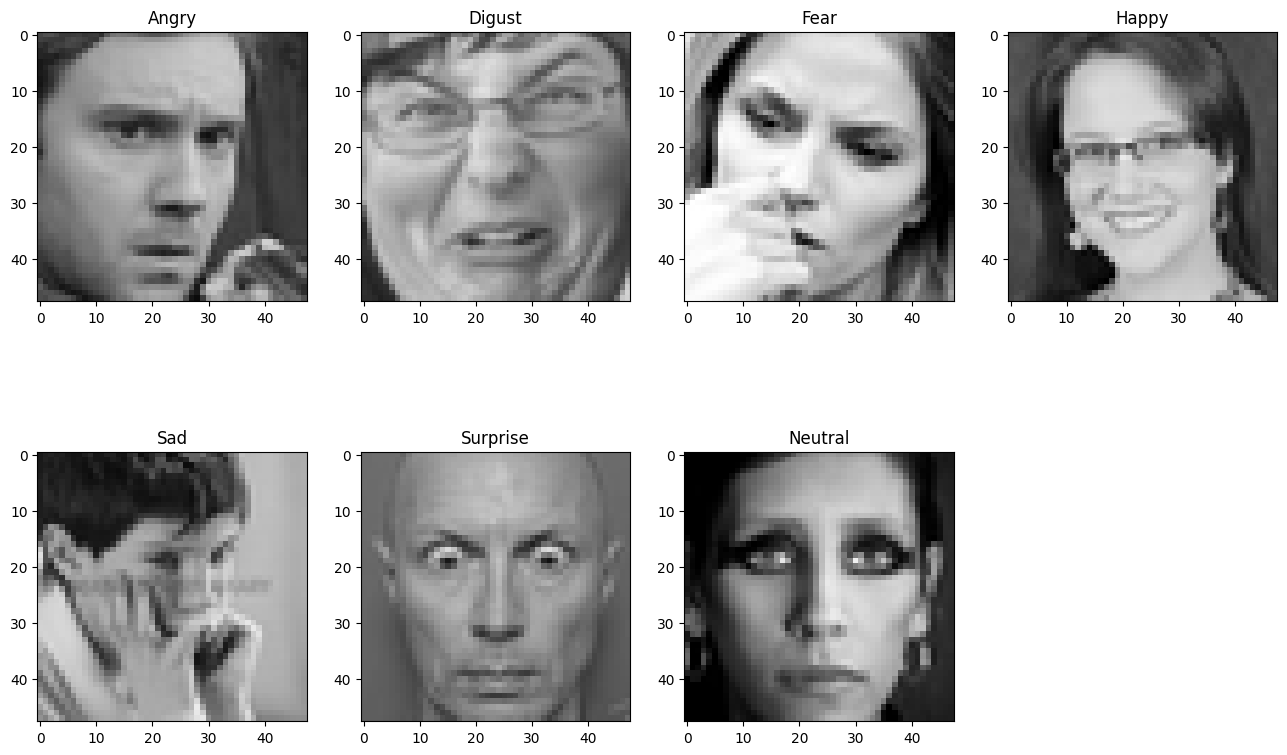
\includegraphics[width=10cm]{Images/fer2013.png}
    \caption{FER-2013 Dataset}
    \label{fig:fer2013}
\end{figure}
A dataset capable of precisely capturing a wide range of human emotions through facial expression was needed for training the model. 
Therefore, the FER-2013 \citep{challenges_in_representation_learning_facial_expression_recognition_challenge} dataset which is a well-known benchmark in the field of  \gls{fer} from the Kaggle competition platform was chosen.
A wide range of facial expressions are included in this dataset, and each of these grayscale images of faces are labelled with one of seven emotions.
This makes it suited for training \gls{fer} models.
\begin{figure}[h!]
    \centering
    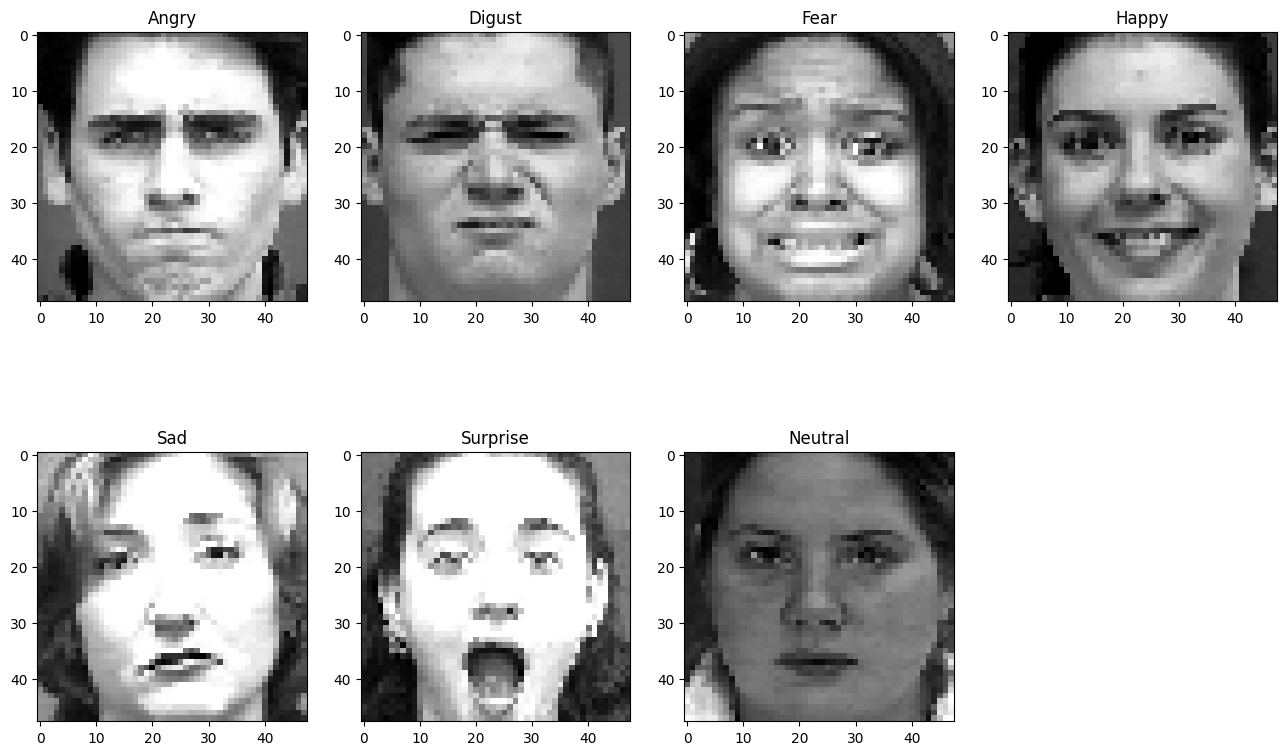
\includegraphics[width=10cm]{Images/ckextended.png}
    \caption{CK+ Dataset}
    \label{fig:ckextended}
\end{figure}
\\
\indent To increase the diversity of the data, CK+ \citep{5543262} dataset is included to the FER-2013. 
This dataset contains labelled facial expressions from varied populations and light scenarios.
This addition was to provide the models a more comprehensive learning environment by exposing them to a greater variety of face emotions and characteristics.
\begin{figure}[h!]
    \centering
    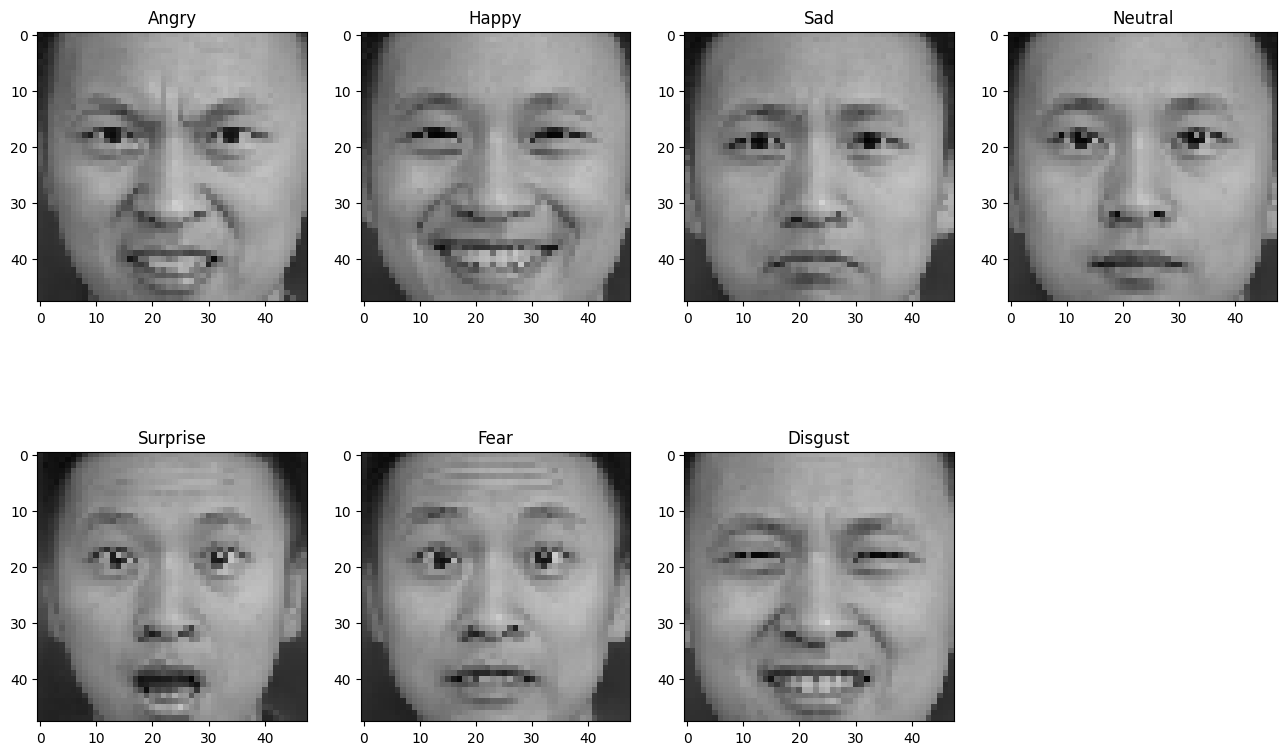
\includegraphics[width=10cm]{Images/szuemodage.png}
    \caption{SZU-EmoDage Dataset}
    \label{fig:szu-emodage}
\end{figure}
\\
\indent Moreover, SZU-EmoDage \citep{who_2022_a} dataset was also included to the collection to ensure the models are capable of identifying facial expressions on Asian faces.
With these additions, each dataset was integrated with a different set of challenges and viewpoints, which then improve the model's accuracy and practicality in real-world situation.
\paragraph{Preprocessing Steps}
Those collected data went through a series of preprocessing stages to standardize input features and optimize them for efficient \gls{ml} before training.
Even though the data were already in grayscale, all images were first converted to grayscale using the \texttt{cv2.cvtColor(image, cv2.COLOR\_BGR2GRAY)} function to ensure that all data were in grayscale in order to simplify the input data and reduce computational cost.
After conversion, all images were shrunk to 48x48 pixels.
It is because neural networks require consistent picture sizes in order to handle batch data efficiently and handle all inputs equally during the learning process.
\\
\indent Following resizing, images were flattened from a format of 2D arrays to a 1D array with 2304 elements (48x48). 
This transformation is necessary because machine learning algorithms generally require a flat array of features for each sample to be handle and analyse.
The flattened image data was then compiled into a pandas DataFrame, which made data handling and analysis in Python simpler.
Before training models, pixel values from each image were standardized to lie within the range of [0,1]. 
This normalization make sure that all input characteristics contribute equally to the model's learning because having different scale will influence the results.
\\
\indent In order to simplify the model and better match the project with its use in music recommendation, the number of emotion categories was cut down from seven to four.
The four categories were kept were `Neutral', `Happy', `Sad' and `Angry'.
These emotions are more easily applied and useful for determining musical mood.
\paragraph{Augmentation}
Keras' function `\texttt{ImageDataGenerator()}' is used to construct a strategic data augmentation process that improved the model's robustness and allowed it to generalize across a variety of face emotions and situations.
The augmentation techniques that were used included random rotation of images up to \(10^\circ\).
This mimics the natural tilts that occur in expressive moments.
Additionally, width and height shifts, which translate images by up to 10\% of their size in both directions.
This helps with situations when faces are not in the center of the frame.
\\
\indent To help the model learn to identify emotions from faces at different camera distances, random zooming was also applied to some of the images.
Moreover, the images were arbitrarily rotated horizontally so that the model could be trained on mirror copies of faces, therefore double the range of face orientations the model saw in the training.
\paragraph{Dataset Splitting}
A key phase in preparing for training and evaluation of \gls{ml} models is splitting the dataset into training, validation, and testing sets. 
The training set was composed from the `Training' data from FER-2013 and the complete CK+ dataset.
This is to increase the model's capacity to generalize across various demographic groups and emotional states by exposing it too a greater variety of facial expressions and environmental factors.
\\
\indent For validation, the `PublicTest' subset of the FER-2013 was used.
This collection is essential for adjusting the hyper-parameters of the model and for providing an unbiased evaluation of the model's fit on the training dataset.
The `PrivateTest' subset of the FER-2013 was used to do the final evaluation of the model's performance.
In addition to the training, validation, and testing data, SZU-EmoDage dataset is used specifically for transfer learning purpose. 
\subsection{Training Process}
\begin{figure}[h!] 
    \centering
\begin{minted}[frame=lines, framesep=2mm, baselinestretch=1.2, fontsize=\footnotesize, linenos]{python}
    param_grid = {
        'conv_1_filters': [32, 64],
        'conv_2_filters': [64, 96, 128],
        'conv_3_filters': [128, 192, 224],
        'conv_4_filters': [128, 160, 224, 256],
        'conv_1_kernel': [3, 6, 8],
        'conv_2_kernel': [3, 5, 8],
        'conv_3_kernel': [3, 5, 8],
        'conv_4_kernel': [3, 5, 8],
        'dropout_1': [0.1, 0.2, 0.4],
        'dropout_2': [0.0, 0.2, 0.3],
        'dropout_3': [0.0, 0.2, 0.3, 0.4],
        'dense_units': [512, 768, 1024],
        'l1_reg': [0.01, 0.001, 0.0001],
        'optimizer': ['adam', 'sgd'],
        'learning_rate': [1e-2, 1e-3, 1e-4], 
        'epochs': [10, 50, 100]
    }
\end{minted}
    \caption{Parameter Grid}
    \label{fig:param_grid}
\end{figure}
In the training process, a common training framework was introduced for both models (Table \ref{tab:cnn-model-1} and Table \ref{tab:cnn-model-2}) to ensure consistency in the methodological approach.
But some specific adjustments to address the unique characteristics of each model is allowed.
The training process started with a thorough grid search to optimize hyper-parameters including dropout rates, kernel sizes, convolutional filter counts, and dense layer unit counts.
Both models shared the same parameter grid as Figure \ref{fig:param_grid}.
This approach made it easier to explore the configuration space in an organized way, ensuring that each model was tuned to perform optimally.
\\
\indent After searching through the parameter grid (Figure~\ref{fig:model-1-grid-result} and Figure~\ref{fig:model-2-grid-result}), the process focuses on configuring each model's architecture to best capture the nuances of facial expression for \gls{fer}.
Model 1 (Table \ref{tab:cnn-model-1}) has a relatively simple architecture, which require careful tuning if dropout rates and filter sizes to balance feature learning against the risk of over-fitting.
Model 2 (Table \ref{tab:cnn-model-2}) has more additional layers to capture a richer set of features before the final classification layer . 
But this led to a more thorough analysis required for the network's depth in relation to its performance on the validation set, which assisted in identifying when to add dropout and how to adjust the pooling layers.  
\\
\begin{figure}[h!] 
    \centering
\begin{minted}[frame=lines, framesep=2mm, baselinestretch=1.2, fontsize=\footnotesize, linenos]{python}
    es = EarlyStopping(monitor='val_accuracy', patience=5, restore_best_weights=True)
\end{minted}
    \caption{Early Stopping}
    \label{fig:earlystopping}
\end{figure}
\\
\indent To prevent over-fitting, early stopping mechanism, which configured as `EarlyStopping' callback (Figure \ref{fig:earlystopping}), is integrated into the training to monitor validation accuracy and automatically halt training if no improvement was detected for five consecutive epochs.
Most important of all, the callback (Figure \ref{fig:earlystopping}) was set to restore the weights form the epoch with the best validation accuracy, ensuring that the model maintained any progress made prior to the plateau.
This approach allows to train the model as long as beneficial, in the meantime, avoiding over-fitting and maintaining the optimal state achieved during training.
\\
\begin{figure}[h!] 
    \centering
\begin{minted}[frame=lines, framesep=2mm, baselinestretch=1.2, fontsize=\footnotesize, linenos]{python}
    steps_per_epoch=len(train_X) / batch_size
\end{minted}
    \caption{Steps per epoch}
    \label{fig:steps_per_epoch}
\end{figure}
\\
\indent Furthermore, the `\texttt{steps\_per\_epoch}' (Figure \ref{fig:steps_per_epoch}) parameter was calculated to ensure that each epoch processed the entire dataset.
With these techniques, early stopping and calculated epoch steps, the models were able to achieve a balance between computational prudence and strong learning.
Consequently, the models were well-positioned for dependable performance in \gls{fer}, having learned from training data efficiently and been prevented from the risk of over-fitting. 
\subsection{Models Evaluation}
Analytical tools such as confusion matrices, accuracy graph over epochs, and classification reports are used to evaluate the effectiveness of the \gls{cnns} models. 
These insights will help in understanding the strengths and weaknesses of the models, and guide future improvements to improve the model's emotional intelligence.

\subsection{Model 1}
\begin{table}[H]
    \centering
    \renewcommand{\arraystretch}{1.5}
    \begin{tabular*}{\textwidth}{
        @{\extracolsep{\fill}}
        l
        S[table-format=1.2]
        S[table-format=1.2]
        S[table-format=1.2]
        S[table-format=4.0]
    }
      \toprule
      \textbf{Category} & {\textbf{Precision}} & {\textbf{Recall}} & {\textbf{F1-score}} & {\textbf{Support}} \\
      \midrule
      Angry & 0.68 & 0.63 & 0.65 & 491 \\
      Happy & 0.86 & 0.89 & 0.87 & 879 \\
      Sad & 0.61 & 0.54 & 0.57 & 594 \\
      Neutral & 0.62 & 0.71 & 0.66 & 626 \\
      \midrule
      Accuracy & & & 0.71 & 2590 \\
      Macro avg & 0.69 & 0.69 & 0.69 & 2590 \\
      Weighted avg & 0.71 & 0.71 & 0.71 & 2590 \\
      \bottomrule
    \end{tabular*}
    \caption{Model 1 Classification Report}
    \label{tab:m1-class-report}
\end{table}
In the classification reports (Table~\ref{tab:m1-class-report} and Table~\ref{tab:m2-class-report}), the precision, recall, and F1-score for each emotion category provide insights into model performance for each specific emotion.
While evaluating the performance of Model 1, the classification report (Table~\ref{tab:m1-class-report}) shows that the `Happy' emotion achieved the highest precision of 0.86.
It indicates a high ratio of correctly predicted happy instances relative to all predictions for happiness. 
Additionally, the recall for `Happy' is 0.89, showing that the model is adept at identifying true happy states from the test data.
With a balanced recall and prevision, the `Neutral' category has an F1-score of 0.66, indicating an excellent performance in identifying neutral emotions.
The model's overall accuracy is 0.71 meaning that 71\% of predictions were accurate.
\\
\begin{figure}[H]
    \centering
    \subfloat[\centering Model 1 Accuracy Variation \label{fig:model-1-acc-var}]{{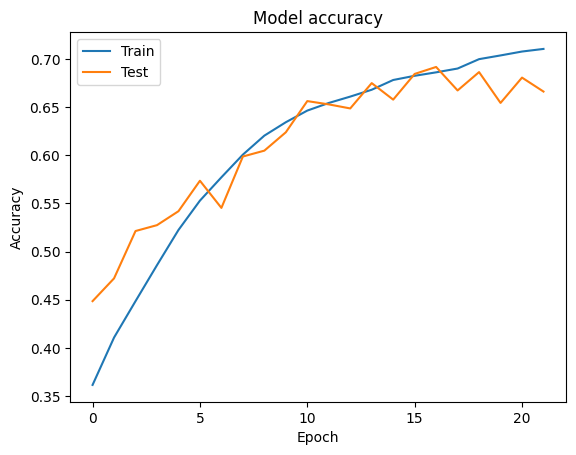
\includegraphics[width=7cm]{Images/model-1-graph.png}}}%
    \qquad
    \subfloat[\centering Model 1 Confusion Matrix \label{fig:model-1-cm}]{{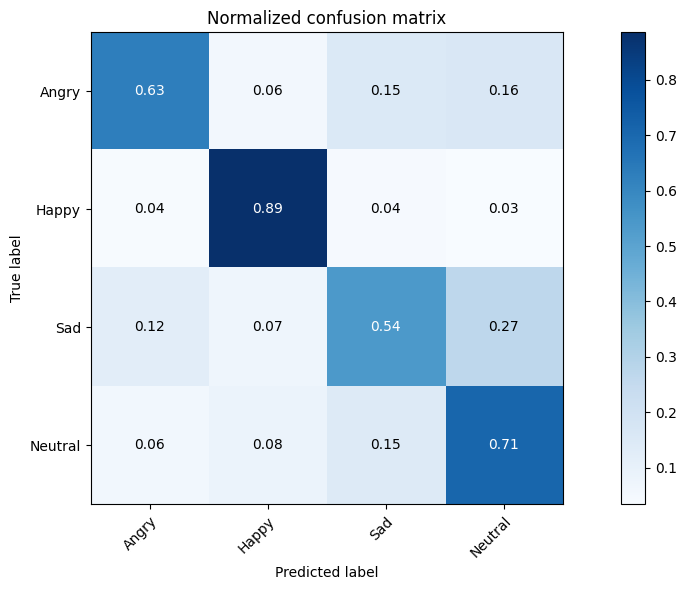
\includegraphics[width=6.7cm]{Images/model-1-conf-mat.png}}}%
    \vspace{0.5cm}
    \\
    \scriptsize{Model 1 Graphs}
\end{figure}
\indent The normalized confusion matrices (Figure~\ref{fig:model-1-cm} and Figure~\ref{fig:model-2-cm}) offers a visual and numerical representation of the model's performance, highlighting correct predictions along the diagonal and errors elsewhere.
Confusion matrices provide a clear view of both true positives and true negatives, which indicate instances in which the model accurately identified the emotional states, as well as false positives and false negatives, which indicate instances in which the model confused one emotion for another.
The diagonal values (Figure~\ref{fig:model-1-cm}) show the percentage of true positives, with `Happy' and `Neutral' emotions have higher values, at 0.89 and 0.71, respectively, suggesting that the model is more confidence in recognizing these emotions correctly.
But, there are some misclassifications, for example, `Angry' being misclassified as `Sad' or `Neutral', and `Sad' being confused with `Neutral'. 
These off-diagonal parts shows where more training data or fine-tuning are required to improve the model's ability to distinguish between emotions with small facial expression differences. 
\\
\indent 
Accuracy graphs (Figure~\ref{fig:model-1-acc-var} and Figure~\ref{fig:model-2-acc-var}) plot the models' performance over each training epoch for both the training and validation datasets.
The graphs provide a clear picture of how the model improves or plateaus over time. 
The graphs also demonstrate the general trend that provides insights about the model's stability and learning capability, as well as the difference in accuracy between training and validation, which shows potential over-fitting.
When the accuracy on the validation is noticeably lower than on the training set, this could be a sign of over-fitting, showing that the model may not generalize well to new data. 
\\
\indent From Figure \ref{fig:model-1-acc-var}, the training dataset shows a noticeable improvement in accuracy with time, showing that model's capacity to pick up knowledge and get better at it.
But, following some initial fluctuations, the test accuracy starts to plateau at about epoch 5, indicating that the model's learning has reached a stable state.
This plateau can indicate that the model has learned as much as it can with the provided architecture and dataset. 
These insights give a thorough understanding of Model 1's performance and suggest possible improvements, including using data enrichment or model refinement to solve misclassifications.

\subsubsection{Model 2}
\begin{table}[H]
    \centering
    \renewcommand{\arraystretch}{1.5}
    \begin{tabular*}{\textwidth}{
        @{\extracolsep{\fill}}
        l
        S[table-format=1.2]
        S[table-format=1.2]
        S[table-format=1.2]
        S[table-format=4.0]
    }
      \toprule
      \textbf{Category} & {\textbf{Precision}} & {\textbf{Recall}} & {\textbf{F1-score}} & {\textbf{Support}} \\
      \midrule
      Angry & 0.73 & 0.62 & 0.67 & 491 \\
      Happy & 0.91 & 0.91 & 0.91 & 879 \\
      Sad & 0.70 & 0.52 & 0.60 & 594 \\
      Neutral & 0.60 & 0.82 & 0.69 & 626 \\
      \midrule
      Accuracy & & & 0.74 & 2590 \\
      Macro avg & 0.74 & 0.72 & 0.72 & 2590 \\
      Weighted avg & 0.75 & 0.74 & 0.74 & 2590 \\
      \bottomrule
    \end{tabular*}
    \caption{Model 2 Classification Report}
    \label{tab:m2-class-report}
\end{table}
The classification report (Table~\ref{tab:m2-class-report}) shows that the model performs well in identifying `Happy' expressions, with high precision (0.91) and recall (0.91) for the `Happy' category.
The precision of `Neutral' is relatively lower at 0.60, indicating some misclassifications.
`Angry' and `Sad' emotions show balanced precision and recall, which indicate that there is still potential for development in accurately identifying these emotions.
\begin{figure}[H]
    \centering
    \subfloat[\centering Model 2 Accuracy Variation \label{fig:model-2-acc-var}]{{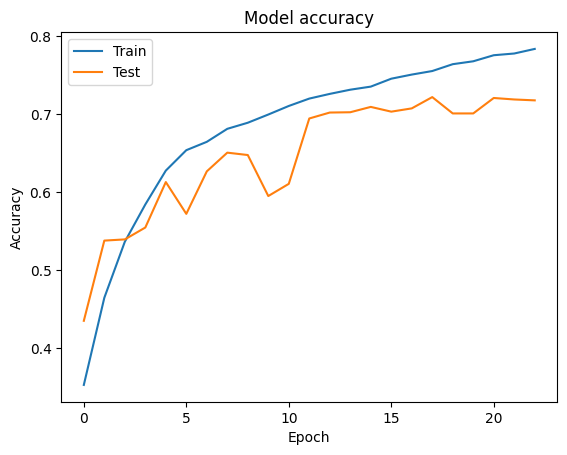
\includegraphics[width=7cm]{Images/model-2-graphs.png}}}%
    \qquad
    \subfloat[\centering Model 2 Confusion Matrix \label{fig:model-2-cm}]{{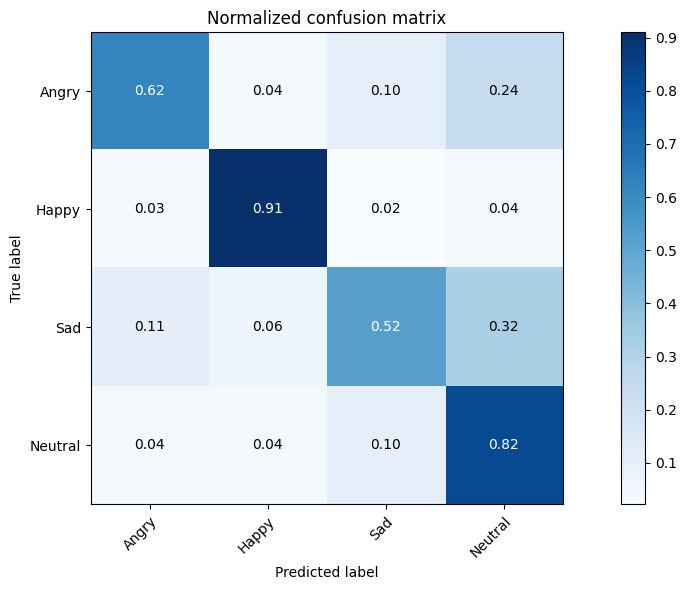
\includegraphics[width=6.7cm]{Images/model-2-conf-mat.png}}}%
    \vspace{0.5cm}
    \\
    \scriptsize{Figure Collection: Model 2 Graphs}
\end{figure}
\indent These findings are further supported by the confusion matrix (Figure~\ref{fig:model-2-cm}), which shows the model's capacity to accurately identify `Happy' and `Neutral' emotions with higher confidence.
These categories are indicated by darker shades along the diagonal.
The off-diagonal figures in the `Angry' and `Sad' sections, with the lighter shades, shows confusion, mainly with `Neutral' expressions.
\\
\indent Training and testing accuracy both steadily rise across epochs in the accuracy graph (Figure~\ref{fig:model-2-acc-var}).
The test accuracy plateaus at about the 15th epoch, indicating that continued training beyond this may not produce meaningful gains and may even worsen over-fitting problems.
\\
\indent All of these results shows that although Model 2 is quite good at identifying `Happy', it struggles to identify `Angry' and `Sad'.
These issues could be resolved by improving the model's generalizability by additional model tuning or data augmentation techniques.

\subsection{Model Comparison and Selection}
\begin{table}[H]
    \centering
    \renewcommand{\arraystretch}{1.5}
    \begin{tabular*}{\textwidth}{@{\extracolsep{\fill}}lcr}
    \toprule
    \textbf{Property} & \textbf{Model 1} & \textbf{Model 2} \\
    \midrule
    Input shape & 48 x 48 x 1 & 48 x 48 x 1 \\
    Weight layers & 6 & 10 \\
    Conv layers & 4 & 7 \\
    Kernel size & 3x3 & 3x3 \\
    Training params & 32,113,028 & 56,303,556 \\
    Model size (MB) & 367 & 644 \\
    Accuracy (\%) & 71.35 & 74.32 \\
    \bottomrule
    \end{tabular*}
    \caption{Comparison of Model 1 with Model 2}
    \label{tab:comparison-models}
\end{table}
The performance of Model 1 and Model 2 is weighted to determine which is more suitable for deployment in this section.
In addition to these variables, recall, accuracy, precision, and the F1-score for every emotional category, the architecture of the model, which depended on computational resources, is also taken into account in this decision making stage. 
\\
\indent The comparative analysis between Model 1 and Model 2 (Table~\ref{tab:comparison-models}) shows that Model 1 with fewer weight and convolutional layers, has much smaller in megabytes and has less training parameters compare to Model 2 which has more complex layers and greater model size.
Besides, Model 2 achieves higher accuracy, which is an important consideration when choosing a model.
It is because the project's objective is to accurately recognizing user's emotional states in order to provide music therapy. 
\\
\indent Although Model 1 has the advantage of being a lighter model which may be beneficial in environments where computational resources are limited, the higher accuracy of Model 2 cannot be disregarded.
The additional complexity of Model 2 is justified given the significance of accurate emotion detection in the context of the web application.
\\
\indent The decision between Model 1 and Model 2 will ultimately come down to balancing accuracy and computational efficiency.
Despite its larger size and more parameters, Model 2 is the better option in terms of giving the best possible music therapy experience since its improved accuracy is more important in achieving the intended user experience.
Therefore, Model 2 is chosen, with further research and development to be done on optimization and efficiency issues.
\\
\subsection{Transfer Learning}
Transfer learning, an approach that repurpose a pre-trained model for a different but related task, is implemented to fine-tune the selected Model 2 for better recognition of Asian facial features, which are underrepresented in the dataset primarily used for training - FER2013 (Figure~\ref{fig:fer2013}) and CK+ (Figure~\ref{fig:ckextended}).
The integration of Szu-EmoDage (Figure~\ref{fig:szu-emodage}) aimed to address and improve the model's ethnic diversity-related limitations.
\begin{figure}[ht!]
    \begin{minted}[frame=lines, framesep=2mm, baselinestretch=1.2, fontsize=\footnotesize, linenos, breaklines]{python}
    for layer in base_model.layers:
        layer.trainable = True 
    \end{minted}
    \caption{Layer Trainable}
    \label{fig:layer-trainable}
\end{figure}
\\
\indent The transfer learning process involved retraining the model's layers, allowing it to learn from new features.
During the fine-tuning stage, it is recommended to freeze certain layers of the model to preserve the knowledge it has acquired from the original datasets, while others were allowed to adjust their weights to the new data.
However, all layers are set to trainable (Figure~\ref{fig:layer-trainable}) in this instance since Szu-EmoDage's size is significantly smaller than the original dataset which is less likely that it would overwrite the learned features from the original datasets.
\begin{table}[H]
    \centering
    \renewcommand{\arraystretch}{1.5}
    \begin{tabular*}{\textwidth}{
        @{\extracolsep{\fill}}
        l
        S[table-format=1.2]
        S[table-format=1.2]
        S[table-format=1.2]
        S[table-format=4.0]
    }
      \toprule
      \textbf{Category} & {\textbf{Precision}} & {\textbf{Recall}} & {\textbf{F1-score}} & {\textbf{Support}} \\
      \midrule
      Angry & 0.92 & 1.00 & 0.96 & 12 \\
      Happy & 1.00 & 0.92 & 0.96 & 12 \\
      Sad & 1.00 & 1.00 & 1.00 & 12 \\
      Neutral & 1.00 & 1.00 & 1.00 & 12 \\
      \midrule
      Accuracy & & & 0.98 & 48 \\
      Macro avg & 0.98 & 0.98 & 0.98 & 48 \\
      Weighted avg & 0.98 & 0.98 & 0.98 & 48 \\
      \bottomrule
    \end{tabular*}
    \caption{Transferred Learning Model Classification Report}
    \label{tab:tf-class-report}
\end{table}
\indent The updated model attained an impressive accuracy of 0.98, showing its ability to apply the learnt properties to a different demographic.
Additionally, every emotion category had almost perfect precision; the lowest was 0.92 for the `Angry' category and the highest was 1.00 for the `Neutral', `Happy' and `Sad' categories.
This improvement demonstrates how well transfer learning works to include a wider variety of data. 
\\
\begin{figure}[H]
    \centering
    \subfloat[\centering Transferred Learning Model Accuracy Variation \label{fig:tf-acc-var}]{{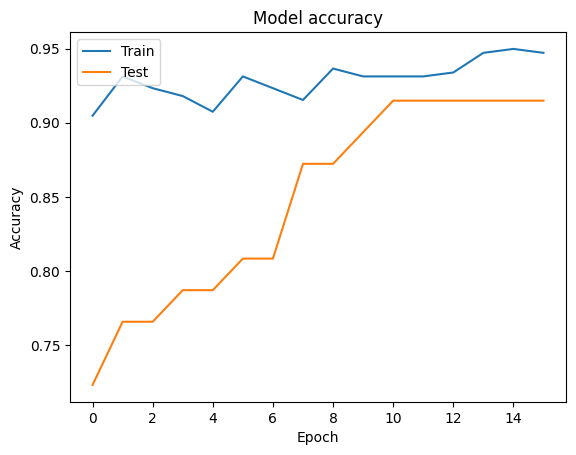
\includegraphics[width=7cm]{Images/tf-graph.png}}}%
    \qquad
    \subfloat[\centering Transferred Learning Model Confusion Matrix \label{fig:tf-cm}]{{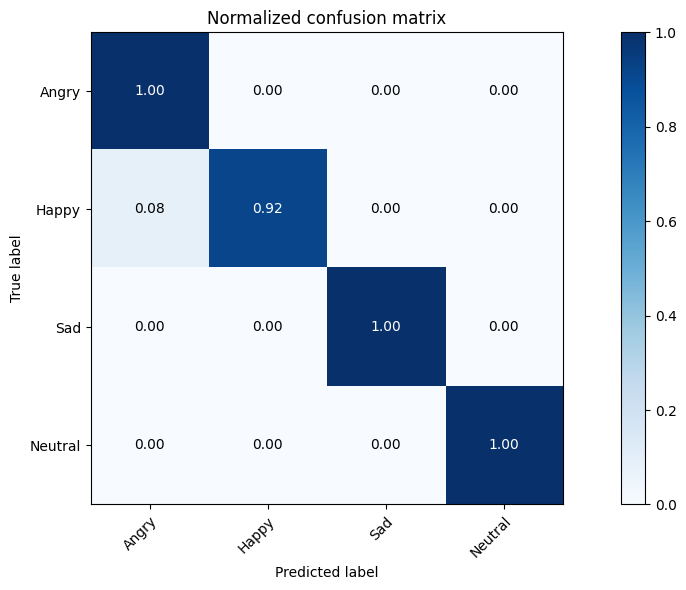
\includegraphics[width=6.7cm]{Images/tf-conf-mat.png}}}%
    \vspace{0.5cm}
    \\
    \scriptsize{Figure Collection: Transferred Learning Model Graphs}
\end{figure}
\indent The model accuracy graph (Figure~\ref{fig:tf-acc-var}), which peaks at 0.99 for the training set, shows a steady training process with high accuracy levels.
The test set accuracy varies notably, but the model still perform well, indicating strong learning without over-fitting.
This prove that the model generalizes the characteristics it has learnt from the original dataset, demonstrating its consistency in performance over varied inputs.
\\
\indent High true positive rates and a clear differentiation between different emotions is showed in the confusion matrix. (Figure~\ref{fig:tf-cm})
Specifically, the model obtained excellent label alignments between the true label and predicted label for the `Angry', `Sad', and `Neutral' categories, resulting in an identification rate of 1.00.
Although there is a small bit of uncertainty with the `Happy' category, which indicates that there is still opportunity for improvement, achieving 0.92 in identifying `Happy' category is still an outstanding result.

\section{Web Application}
\begin{figure}[h!]
    \centering
    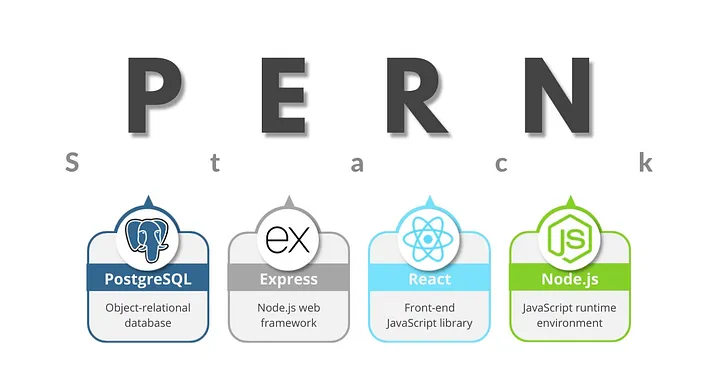
\includegraphics[width=10cm]{Images/pern.png}
    \caption{PERN Stack \citep{alves_2023_get}}
    \label{fig:pern}
\end{figure}
The web application uses the PERN stack (Figure \ref{fig:pern}), which is an acronym for PostgreSQL \citep{thepostgresqlglobaldevelopmentgroup_2019_postgresql}, Express \citep{openjsfoundation_2017_express}, React \citep{metaopensource_2024_react} and Node.js \citep{nodejs_2023_nodejs}.
This set of technologies provides a comprehensive end-to-end foundation for creating dynamic web application.
\\
\indent The frontend was built with React.js, a widely-used \gls{js} \gls{ui} framework, which was chosen for its declarative and effective method of creating \gls{ui}.
For the backend, Node.js was chosen for its non-blocking, event-driven architecture.
This architecture is well-suited for managing workloads that involve asynchronous operations, real-time applications and I/O-bound tasks.
The backend API is then constructed using Express.js, a simple and adaptable Node.js web application framework.
PostgreSQL is the chosen database system as it is well-known for its advanced features, data integrity and robustness.
\subsection{Login and Registration}
\begin{figure}[h!]
    \centering
    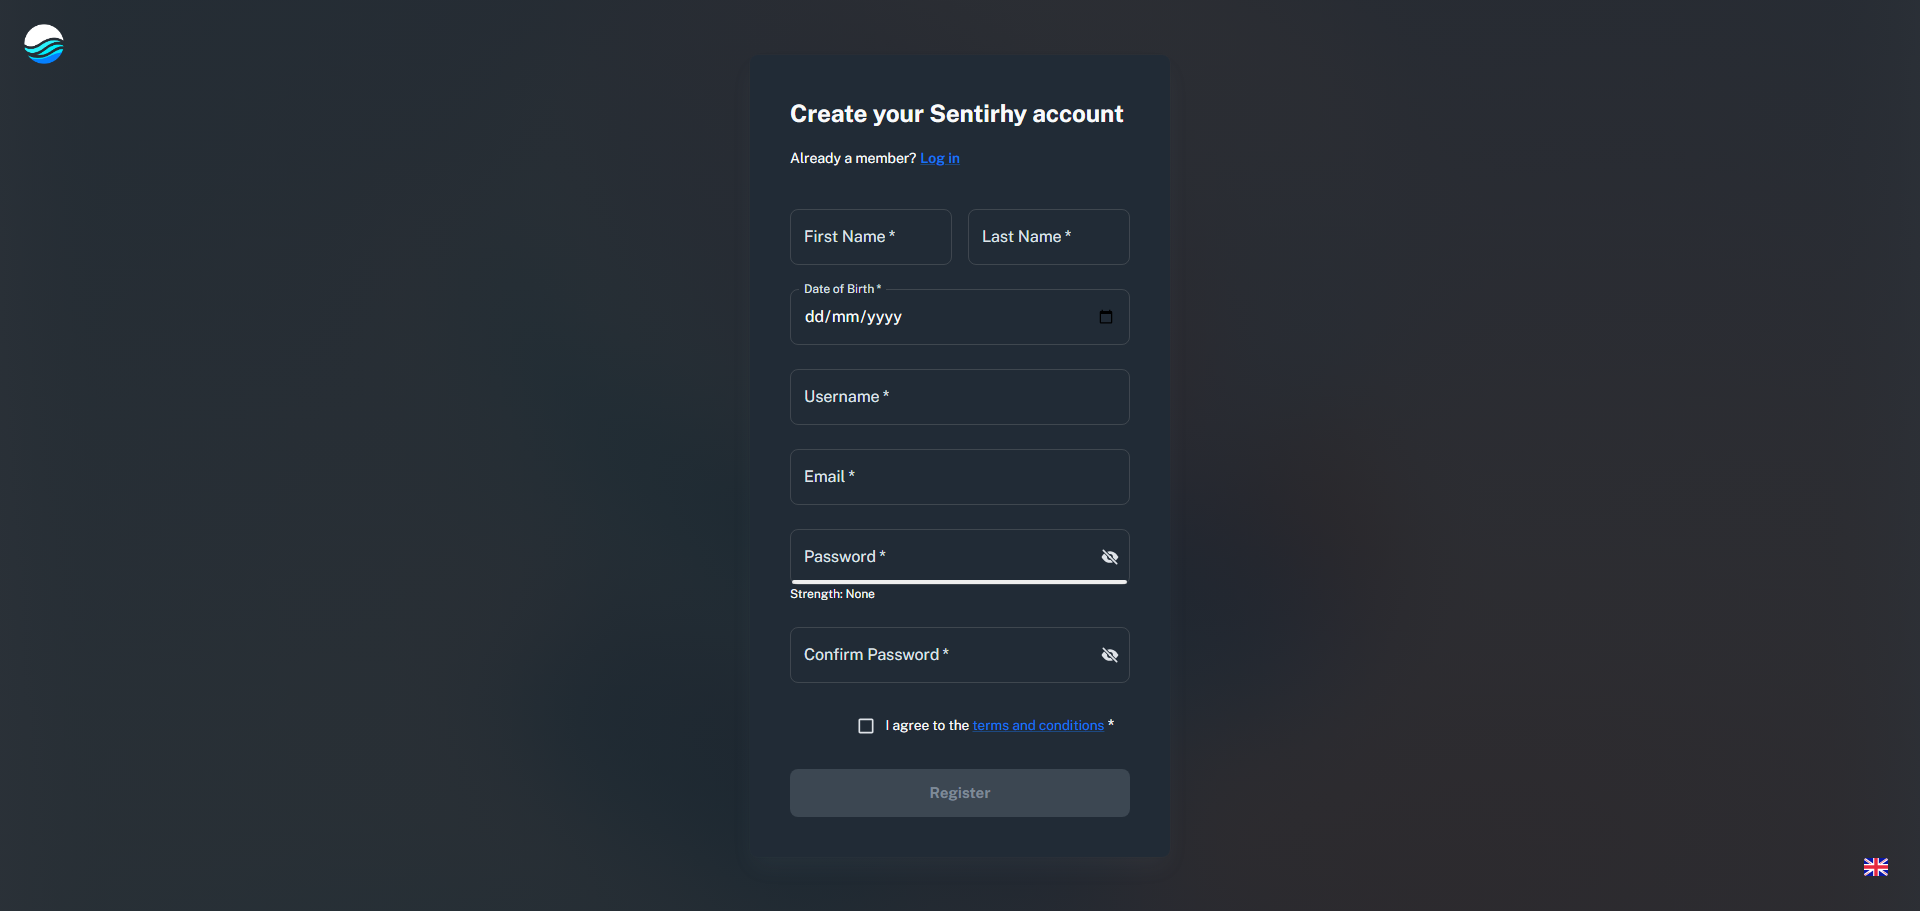
\includegraphics[width=14cm]{Images/register-ui.png}
    \caption{Register Page - UI}
    \label{fig:register-page-ui}
\end{figure}
Users first provide their personal information, which consists of their date of birth, fist and last names, preferred username, and email address, to begin the registration process. (Figure \ref{fig:register-page-ui}) 
The entered data is then validated by cross-referencing it with existing entries in the `sentirhy.user' table within the PostgreSQL database.
If there is duplicated username or email, the user will be notified that the credentials have already been taken and the process will stopped.
When there is no duplicate entry, the user's password is securely hashed with `bcrypt' (Figure~\ref{fig:registering-user} Line 9), and the `crypto' module creates an unique activation token which will then send to the user's email for account verification.
The generated token with an expiration date is also stored in the database with the user credentials for security purposes. 
\\
\begin{figure}[h!]
    \centering
    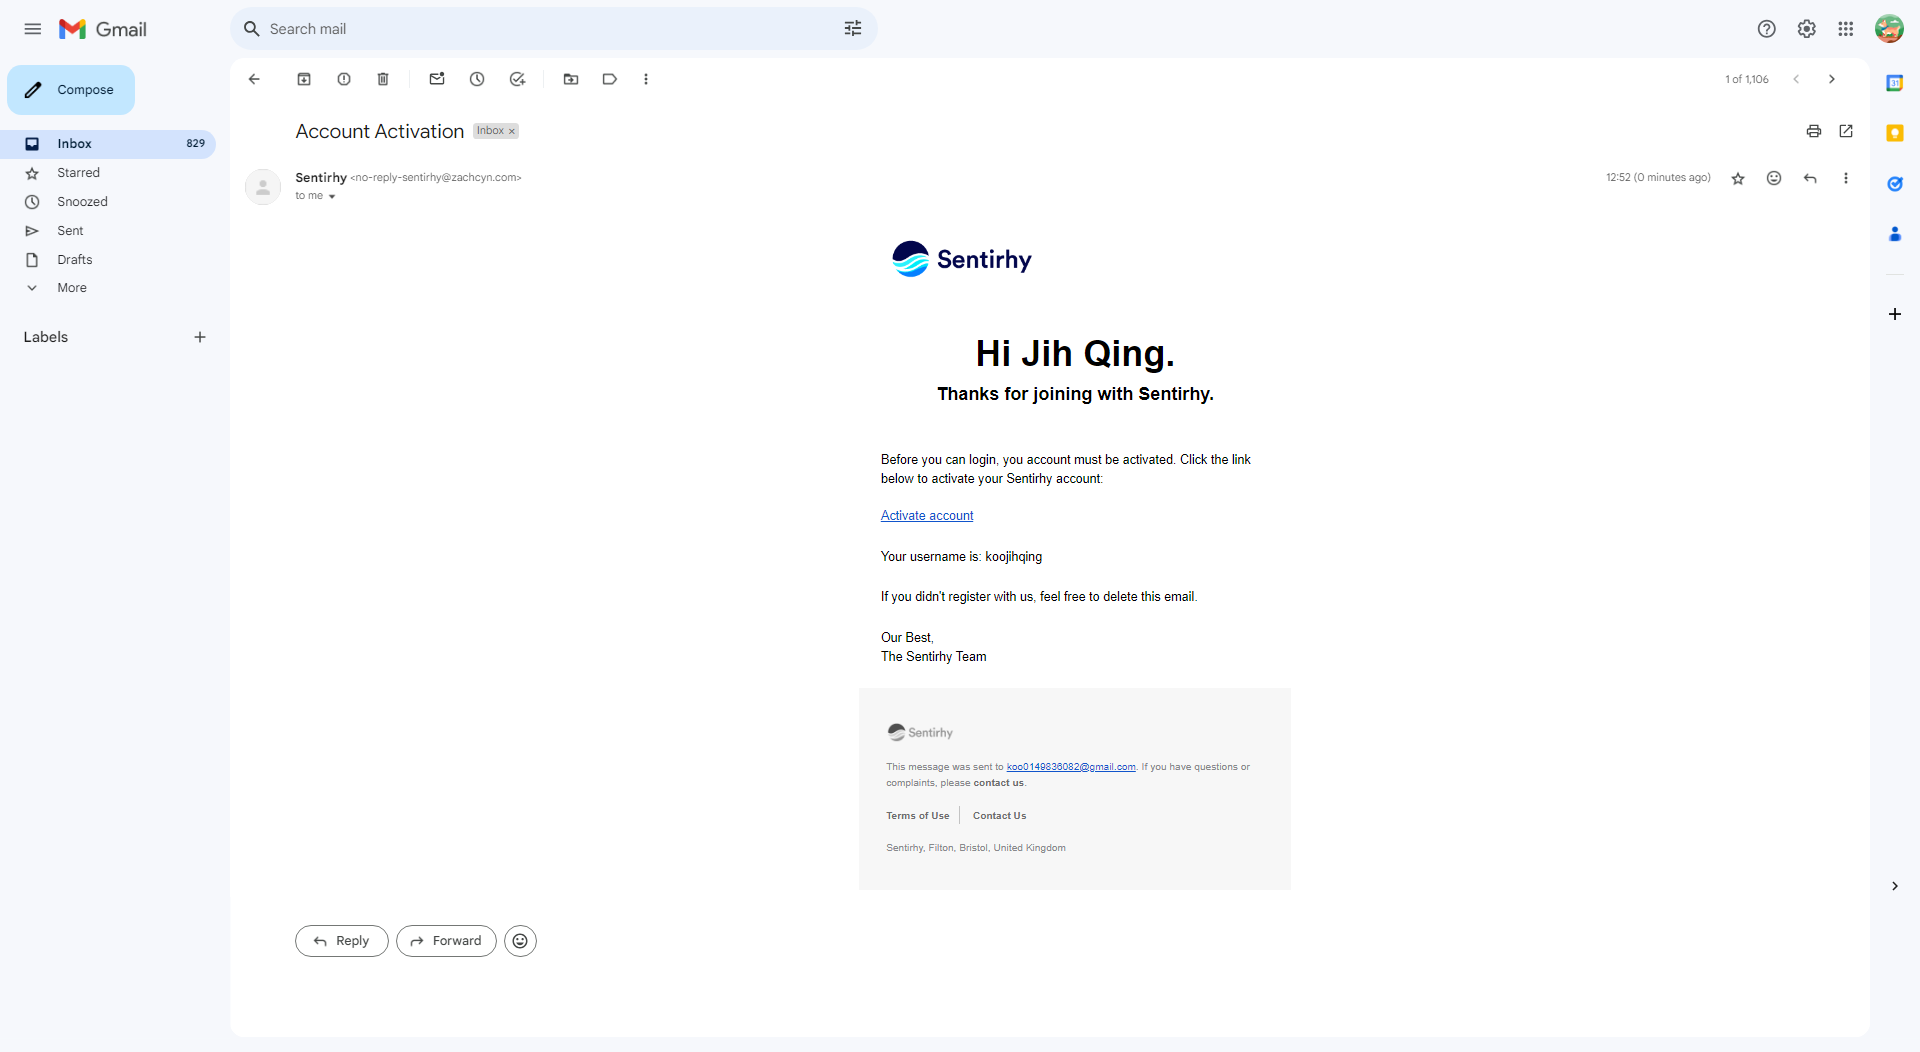
\includegraphics[width=14cm]{Images/acc-activation.png}
    \caption{Account Activation Email - UI}
    \label{fig:account-activation-ui}
\end{figure}
\begin{figure}[h!]
    \centering
    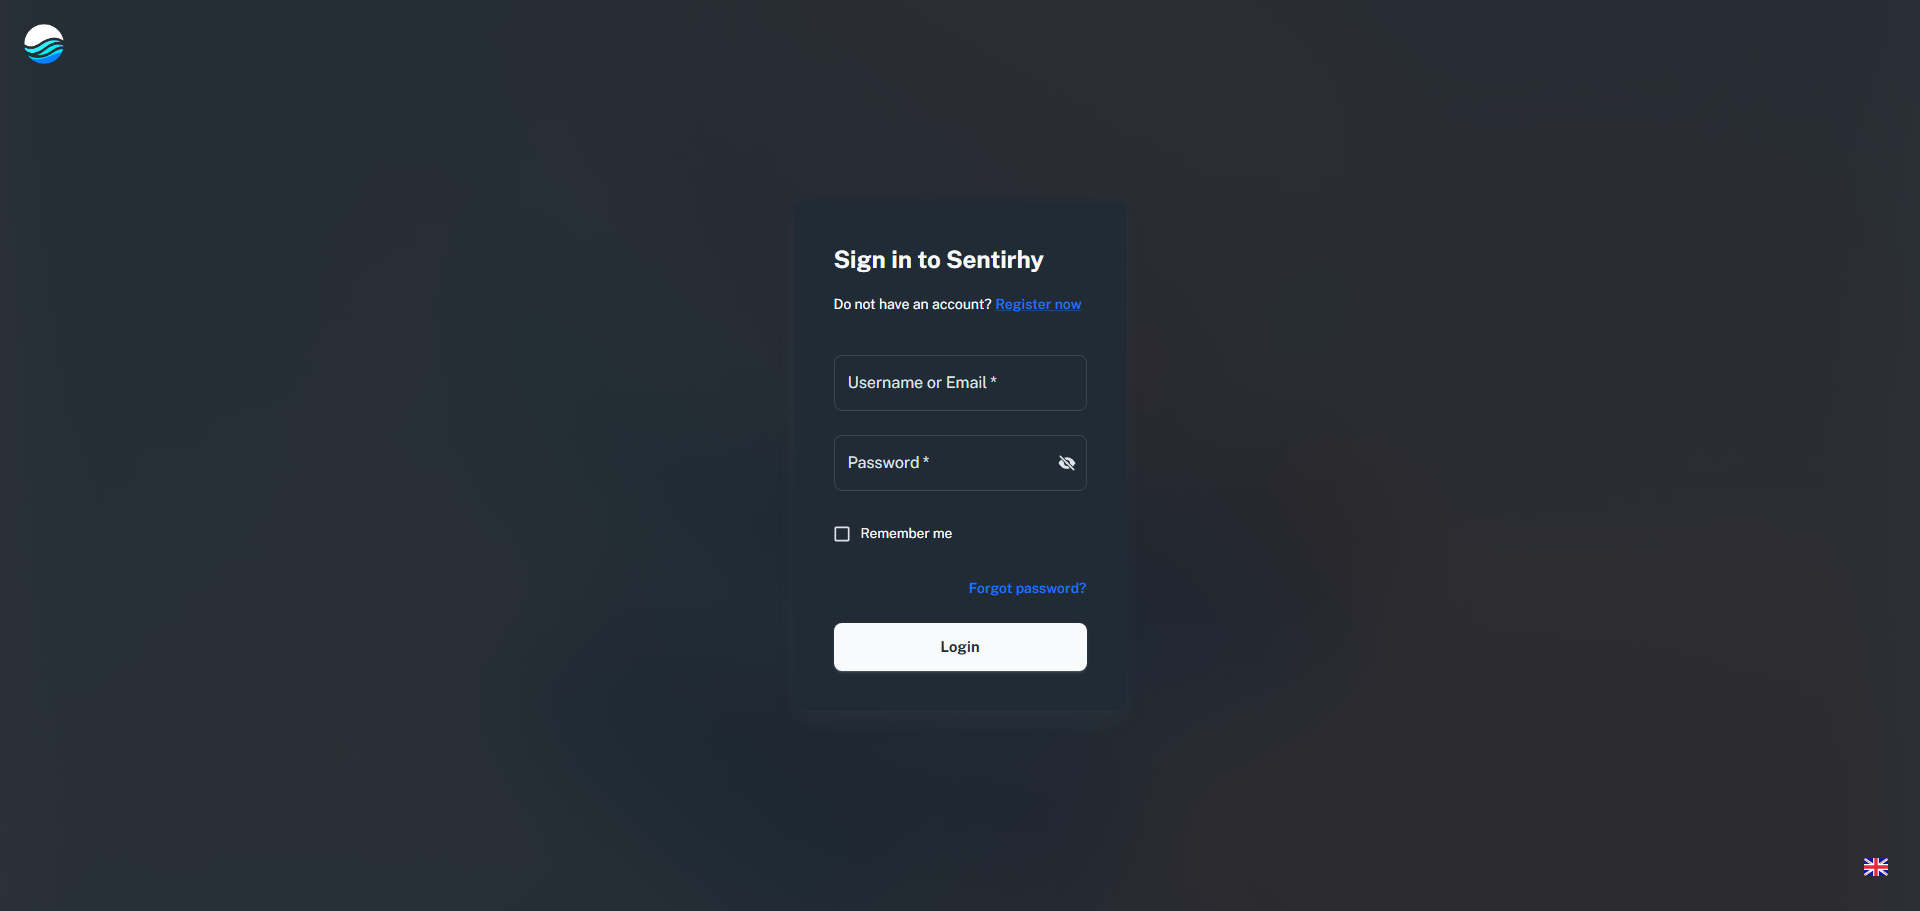
\includegraphics[width=14cm]{Images/login-ui.png}
    \caption{Login Page - UI}
    \label{fig:login-page-ui}
\end{figure}
\\
\indent An activation email (Figure \ref{fig:account-activation-ui}) is sent out using the `nodemailer' after the new user's database entry.
For the login process (Figure \ref{fig:login-page-ui}), the username and password are required.
After user submitted the credentials, the system compares those credentials to those kept in the database. 
Then, access to the application is granted with a successful match and an activated account.
\\
\subsection{Integration with Music Services}
\begin{figure}[h!]
    \centering
    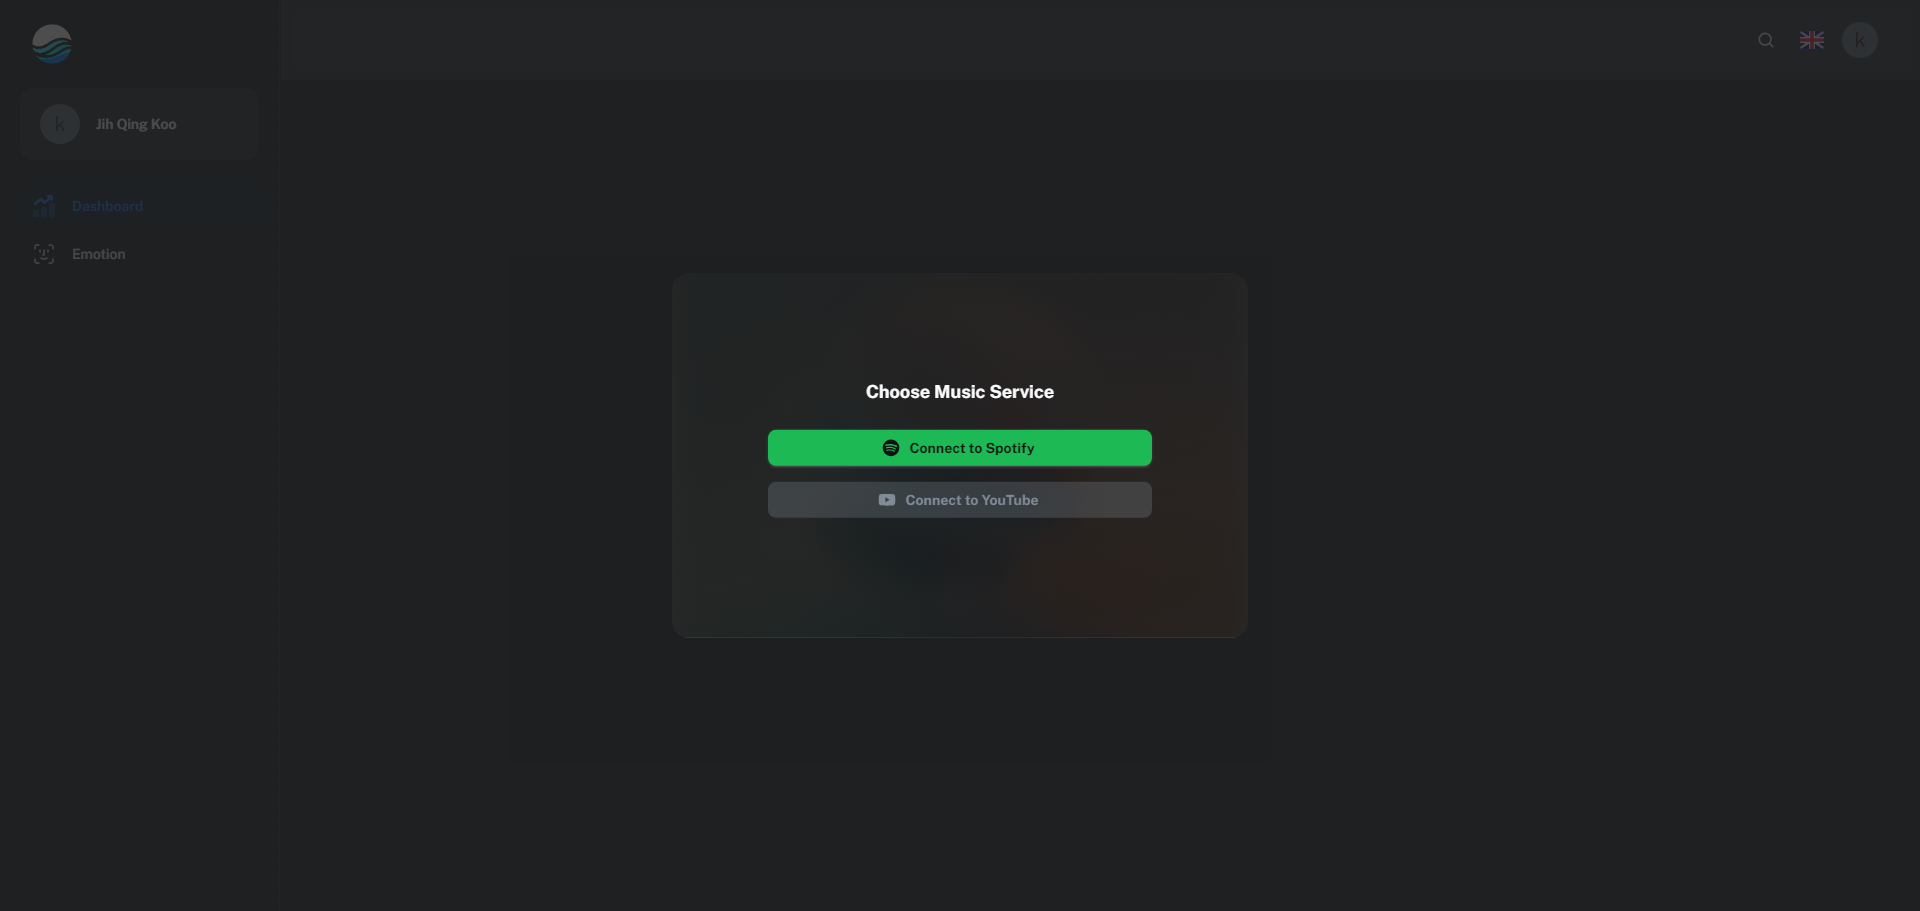
\includegraphics[width=14cm]{Images/connect-api.png}
    \caption{Music Services Connection - UI}
    \label{fig:music-service}
\end{figure}
As users log into the application, they are greeted with a dashboard.
There will be a modal component (Figure~\ref{fig:music-service}) showing on the dashboard, allowing users to connect to different music services, which is required to the app's function to play music.
Users are redirected to Spotify's authorization interface through an OAuth 2.0 authorization flow in order to grant permissions when they choose to link their Spotify accounts.
Once user's permission is acquired, an access token from Spotify's token endpoint gives the application the authority to request services from the Spotify API on the user's behalf, like playing music.
Unfortunately, as of right now, the only integration that is operational is Spotify; Youtube connectivity is indicated as a planned addition.
\\
\subsection{Emotion Detector}
\begin{figure}[h!]
    \centering
    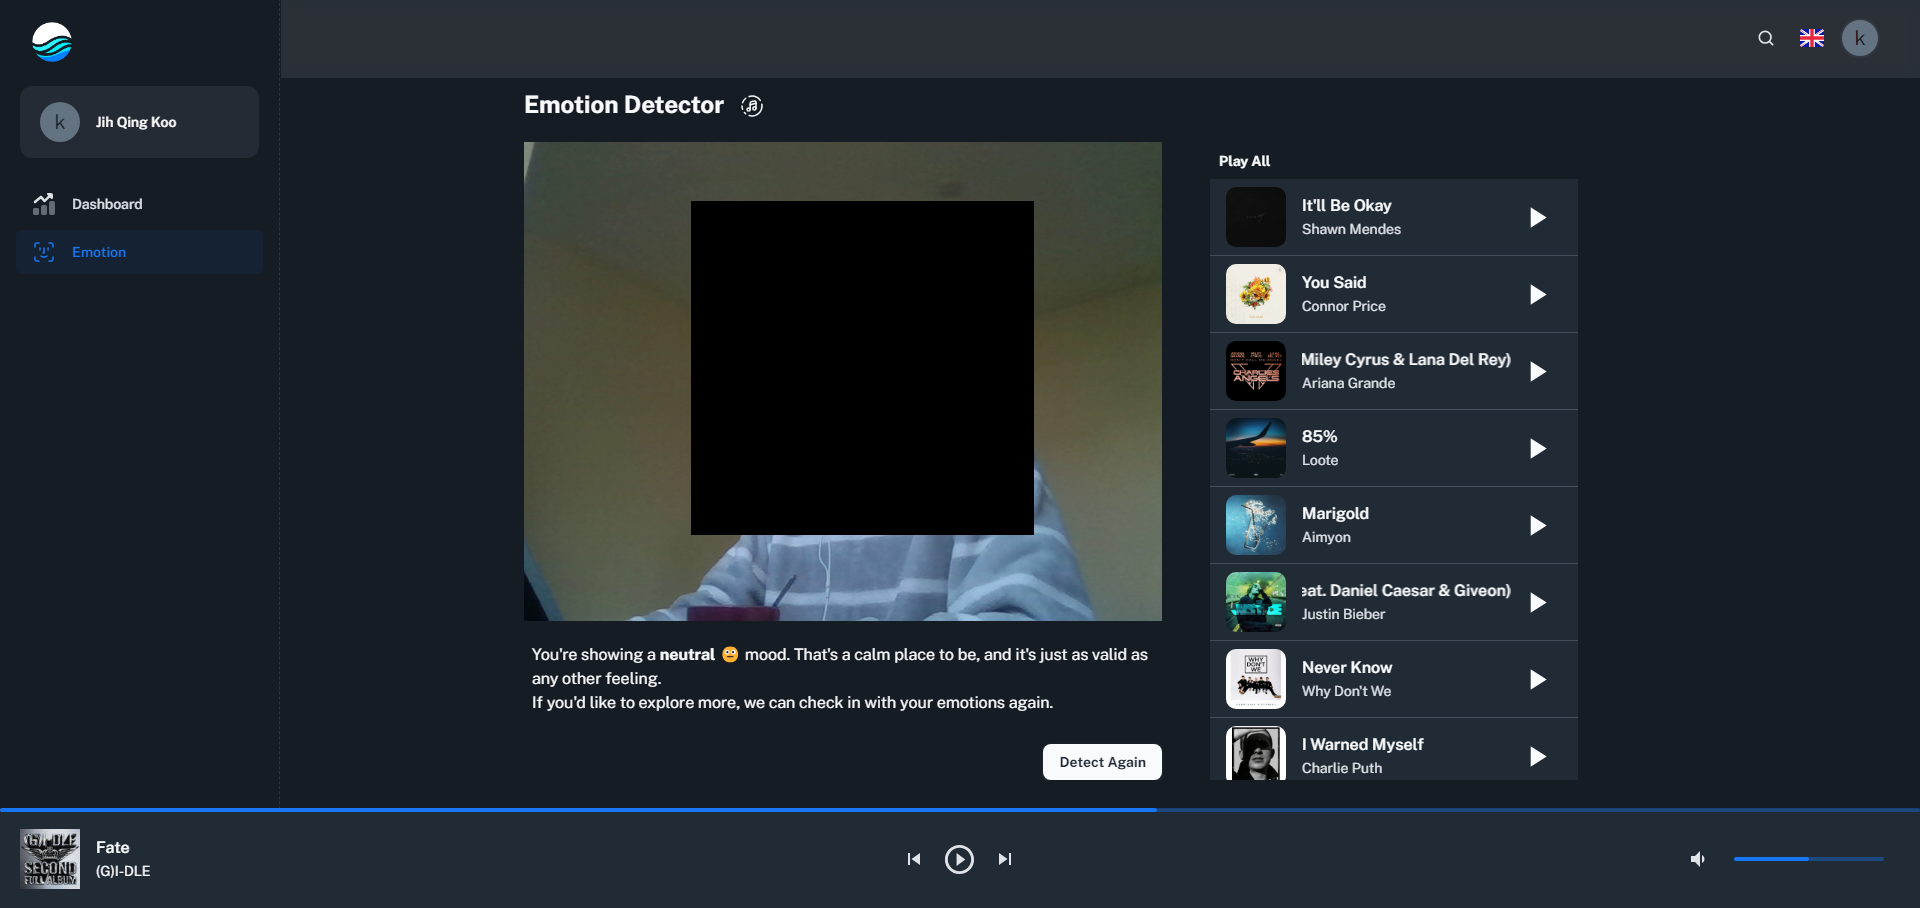
\includegraphics[width=14cm]{Images/emotion-detector.png}
    \caption{Emotion Detector - UI}
    \label{fig:emo-detect}
\end{figure}
When user enters the Emotion Detection page (Figure~\ref{fig:emo-detect}), they encounter an interactive interface that requires access to the camera to proceed.
With the user's permission, the application launches the Haarcascade frontal face identification algorithm and opencv.js, the \gls{js} library of OpenCV, enabling real-time face detection through the live video feed.
\\
\begin{figure}[h!] 
    \centering
\begin{minted}[frame=lines, framesep=2mm, baselinestretch=1.2, fontsize=\footnotesize, linenos, breaklines]{javascript}
    async function predictEmotion(imageFilename) {
        const imagePath = path.join(__dirname, '/user_emotion/', imageFilename);
        const model = await loadModel()
        const imageBuffer = await fs.promises.readFile(imagePath);
        const tensor = tf.node.decodeImage(imageBuffer).resizeBilinear([48, 48]).mean(2).expandDims(-1).expandDims(0).toFloat().div(tf.scalar(255));
        const prediction = model.predict(tensor);
        const emotionIndex = prediction.argMax(1).dataSync()[0];

        return emotions[emotionIndex];
    }
\end{minted}
    \caption{Load Model and Preprocess data}
    \label{fig:load-process}
\end{figure}
\indent The system is designed to identify faces quickly and captures the frame.
The captured frame is then sent to the backend in a binary format appropriate for transmission over the network.
The backend, which has been configured with TensorFlow.js, awaits the binary format data to perform its function.
It loads the trained model, then resize the image to 48x48 pixels, converted to grayscale, normalized to scale the pixel values, and batched for the model's evaluation in order to meet the model's needs. (Figure~\ref{fig:load-process})
\\
\begin{figure}[h!] 
    \centering
\begin{minted}[frame=lines, framesep=2mm, baselinestretch=1.2, fontsize=\footnotesize, linenos, breaklines]{javascript}
    function generateProgressivePlaylist(user_emotion_tracks, neutral_tracks, happy_tracks, playlistLength) {

        const allTracks = user_emotion_tracks.concat(neutral_tracks, happy_tracks);
        allTracks.sort((a, b) => a.valence - b.valence);
        const step = Math.floor(allTracks.length / playlistLength);

        const selectedTracks = [];
        for (let i = 0; i < playlistLength && (i * step) < allTracks.length; i++) {
            selectedTracks.push(allTracks[i * step]);
        }

        return selectedTracks;
    }
\end{minted}
    \caption{Generate Playlist}
    \label{fig:generate-playlist}
\end{figure}
\indent When the image is in an acceptable format, the model starts to recognize the user's current emotional state.
Once the emotion is deciphered, the system responds by creating playlist that corresponds with the feeling. (Figure~\ref{fig:generate-playlist})
The generated playlist is then dynamically displayed on the \gls{ui}.
